\documentclass[]{article}

\usepackage{graphicx}
\usepackage{booktabs}
\usepackage{adjustbox}


% Title Page
\title{IE5202 Project 2 Report}
\author{Yang Xiaozhou, A0113538}


\begin{document}
\maketitle

\section{Exploratory Data Analysis}

The exchange rate from 1980 to 1995 seems to have experienced three distinct phases with a drastic drop around 1986. The three phases are shown in Fig \ref{fig:jpy_usd_three_peridos}.
%
\begin{figure}[hbtp]
	\centering
	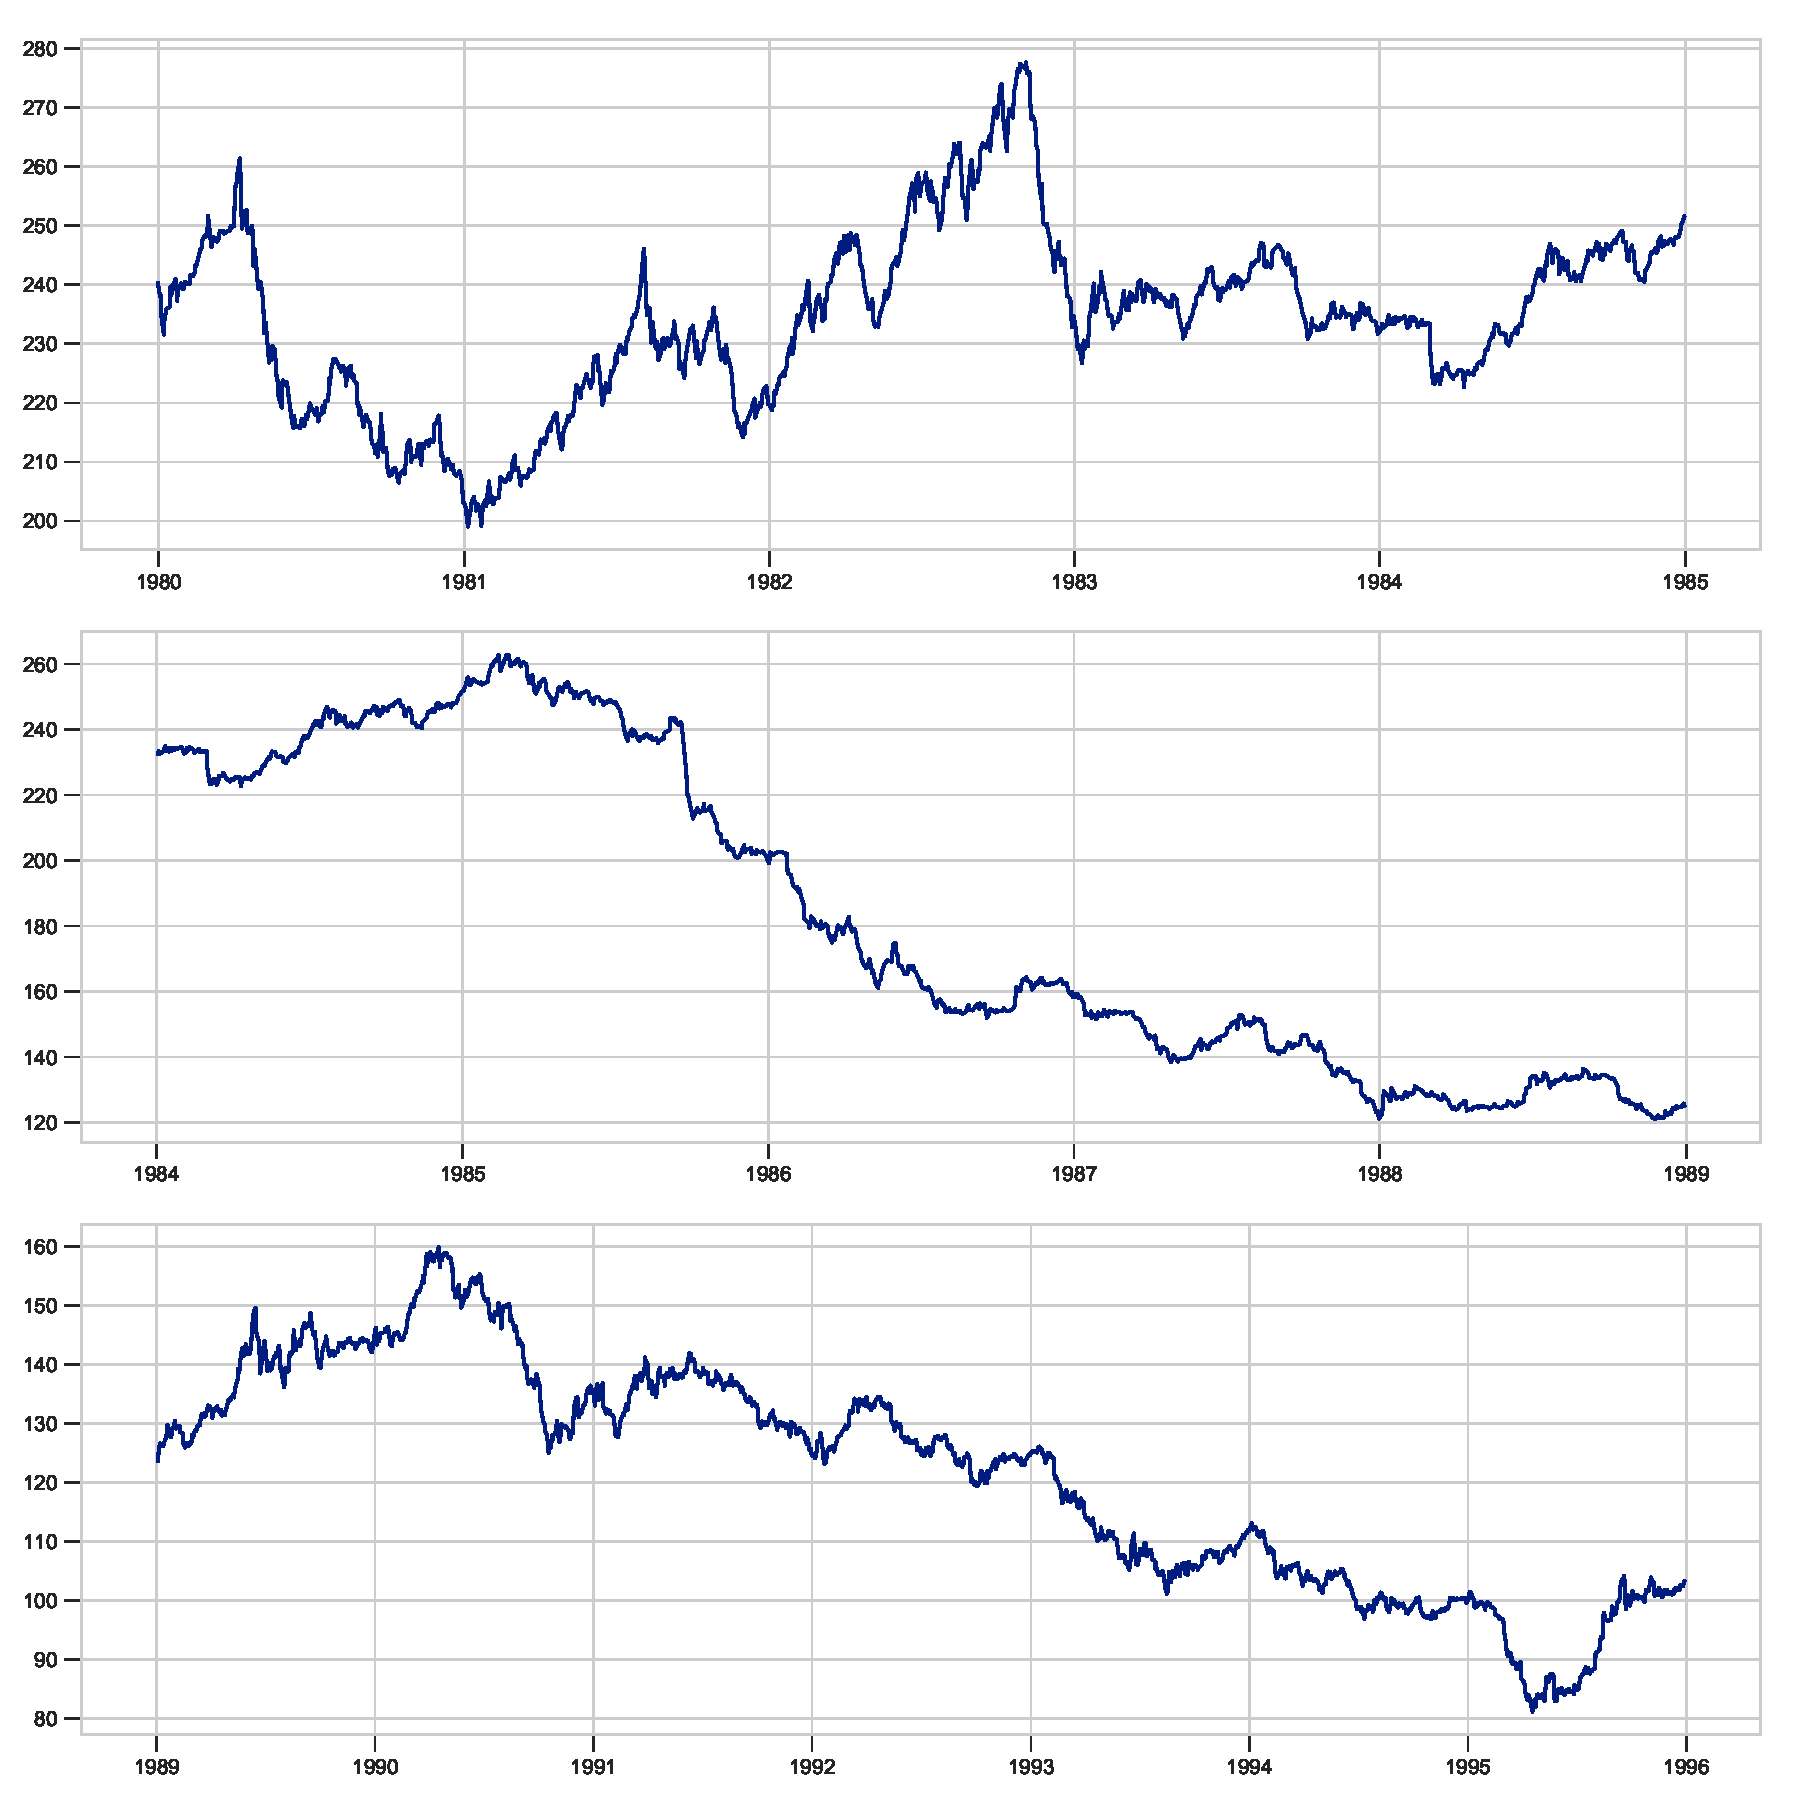
\includegraphics[width=1\columnwidth]{../Figures/jpy_usd_three_periods.pdf}
	\caption{JPY/USD During Three Separate Periods.}
	\label{fig:jpy_usd_three_peridos}
\end{figure}
%
The time series always exhibit strong autocorrelation even beyong 100 lags as shown in Fig \ref{fig:sacf_n_spacf_plot}. SPACF plot shows the lag cuts off after order 1. This indicates an AR(1) model might be appropriate for the time series. 
%
\begin{figure}[hbtp]
	\centering
	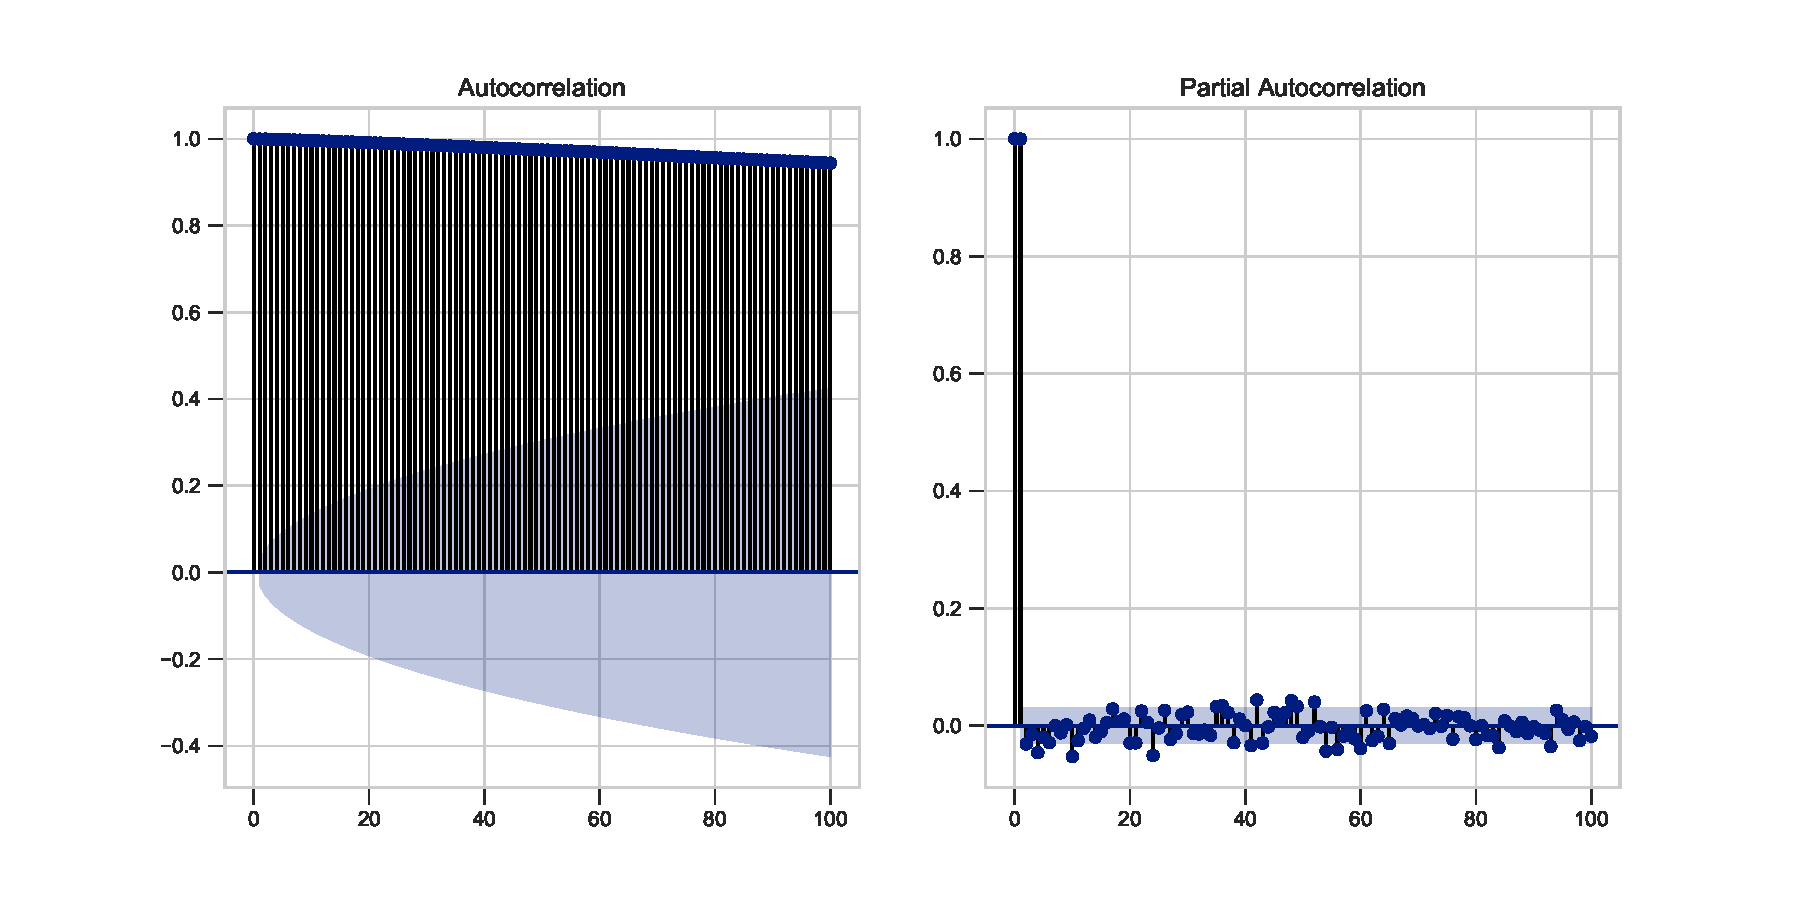
\includegraphics[width=1\columnwidth]{../Figures/sacf_n_spacf_plot.pdf}
	\caption{SACF and SPACF Plot for JPY/USD.}
	\label{fig:sacf_n_spacf_plot}
\end{figure}
%
Judging from the lag plots in Fig \ref{fig:three_lag_plots}, historical values are very good indicators of the future value, at least in the near future (less than 100 days). 
%
\begin{figure}[hbtp]
	\centering
	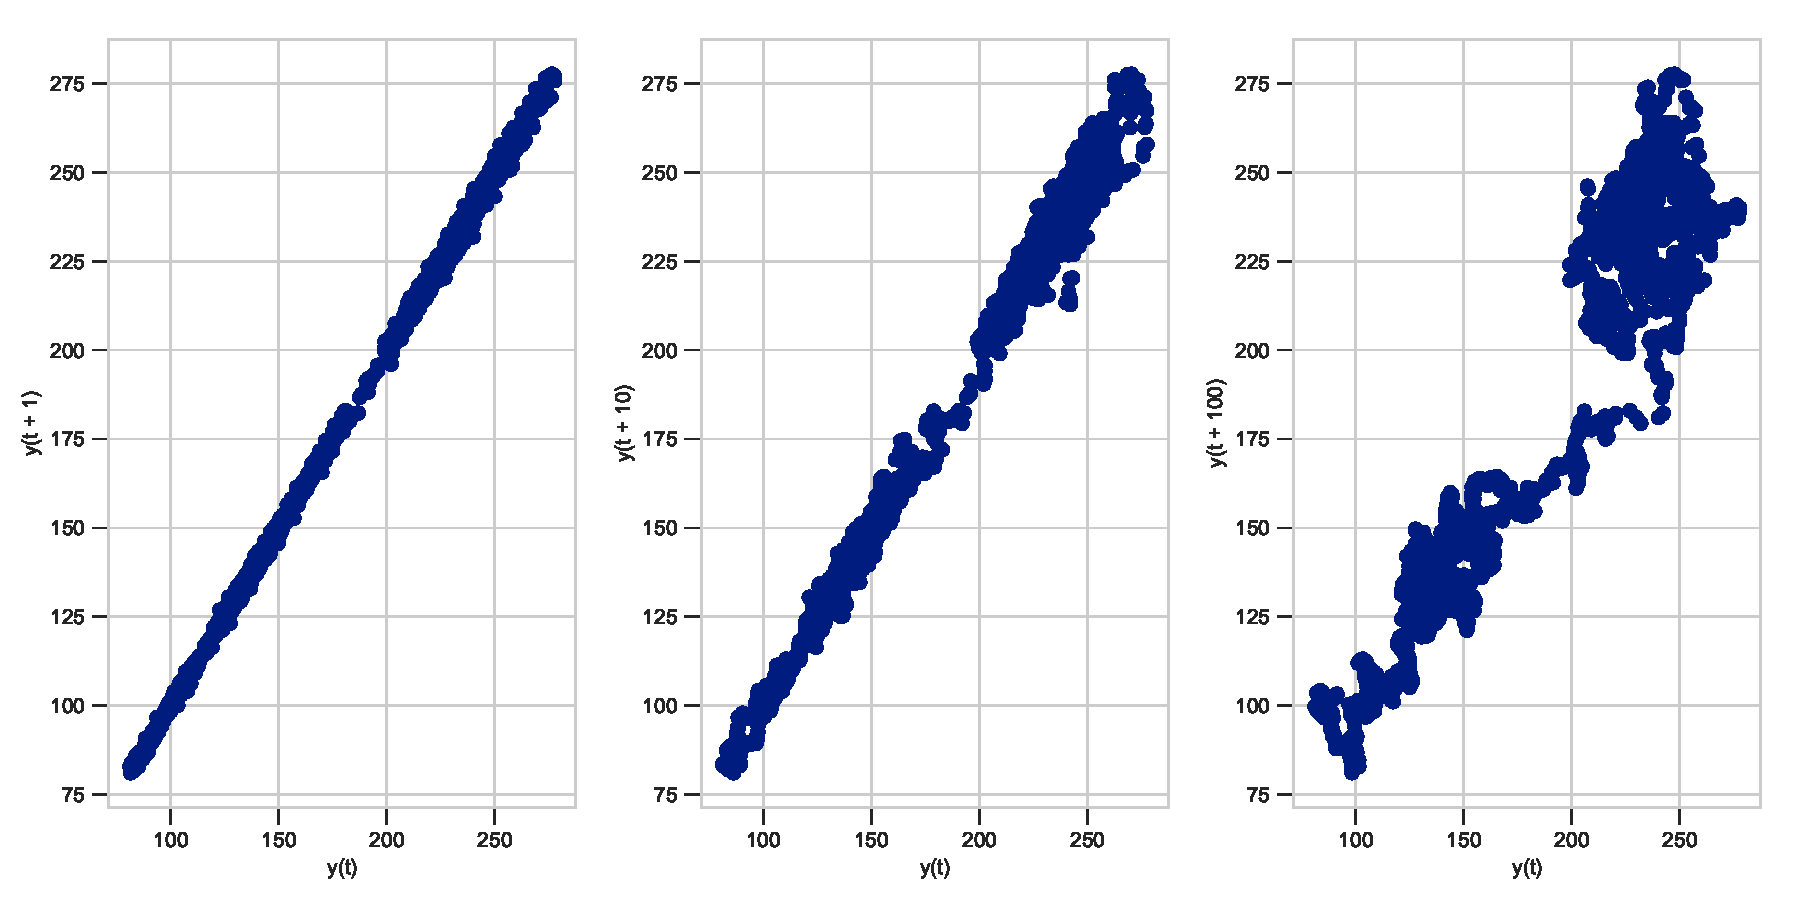
\includegraphics[width=1\columnwidth]{../Figures/three_lag_plots.pdf}
	\caption{Lag Plots at Three Different Level: 1, 10, 100.}
	\label{fig:three_lag_plots}
\end{figure}
%
Also, no obvious seasonal patterns could be observed. 


\section{Model Building}
\subsection{Exponential Smoothing Model}
With exponentially weighted moving average, due to the strong autocorrelation, the optimal smoothing parameter, alpha, is found to be 1 for the smallest root mean square error (RMSE), see Fig \ref{fig:optimal_alpha_ewma}.
%
\begin{figure}[hbtp]
	\centering
	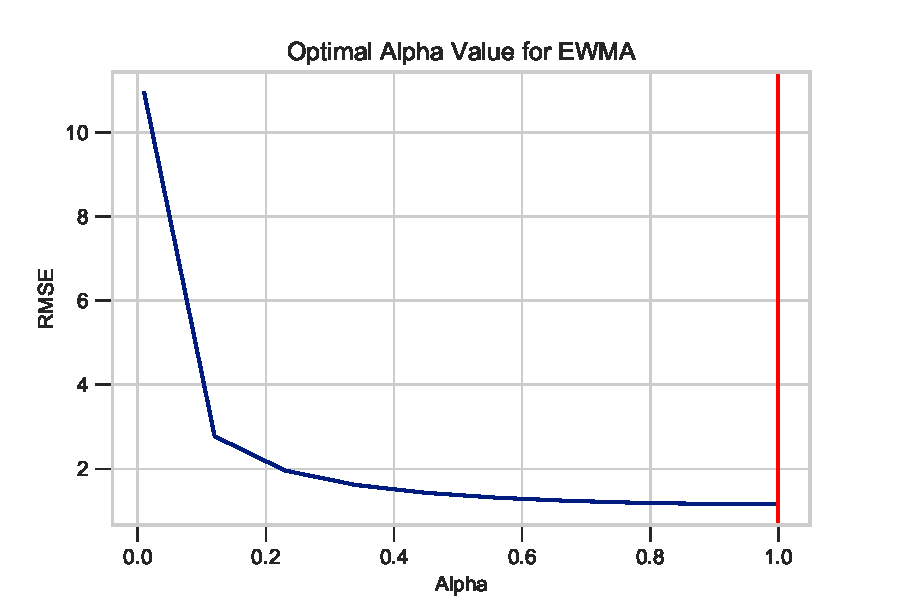
\includegraphics[width=1\columnwidth]{../Figures/optimal_alpha_ewma.pdf}
	\caption{Optimal Alpha.}
	\label{fig:optimal_alpha_ewma}
\end{figure}
%
Similar results are shown when double exponential smoothing model is constructed with the parameter combination of (alpha = 1, beta = 0.12) achieving the least RMSE. 

\subsection{ARIMA Model}
Several ARIMA models are built based on both original data and log-transformed data. 10-fold cross validation RMSEs of 1-step-ahead forecast are reported in Fig \ref{fig:error_estimation_1} for the orginal data and Fig \ref{fig:error_estimation_2} for log-transformed data. For both types of data, AR(1) and MA(1) models on 1st order differencing transformed data perform the best, with the lowest RMSE of 1.048. 

%
\begin{figure}[hbtp]
	\centering
	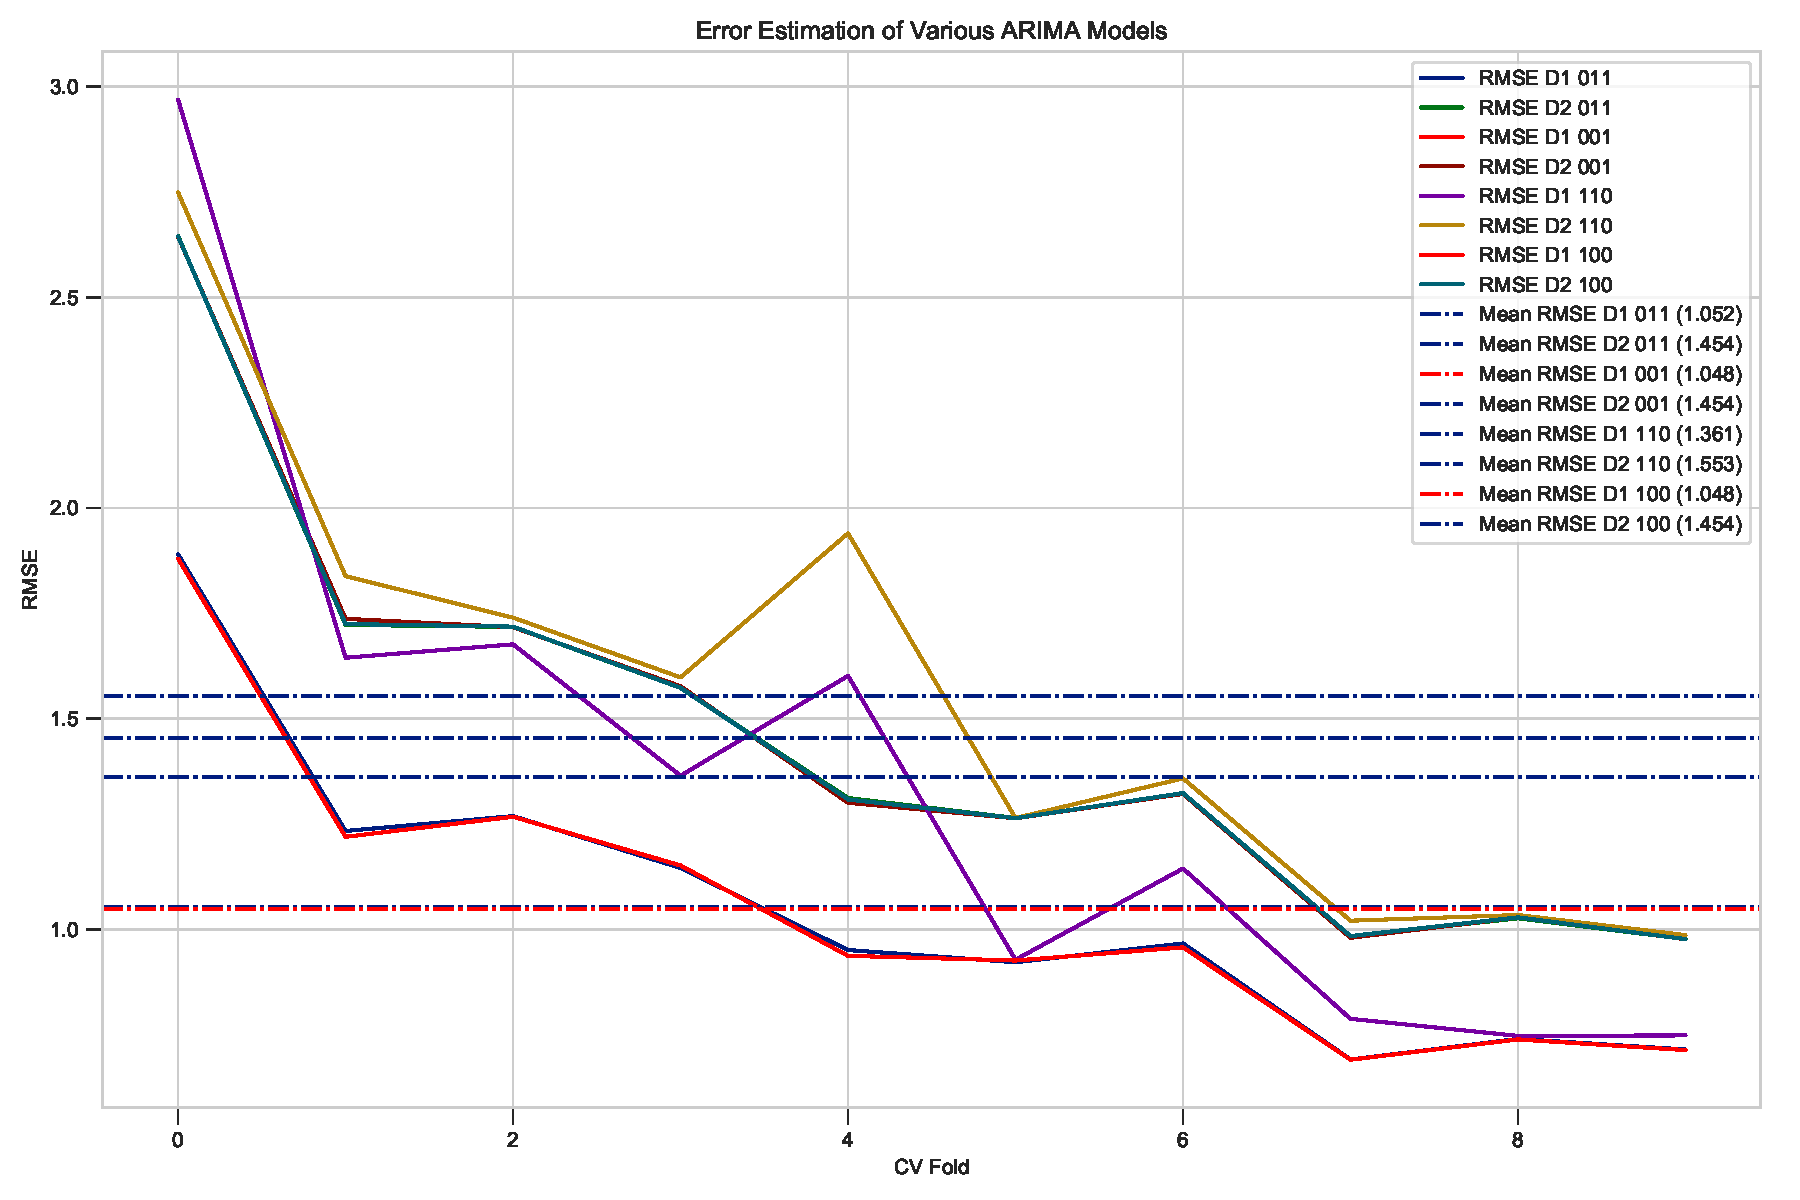
\includegraphics[width=1\columnwidth]{../Figures/error_estimation_1.pdf}
	\caption{Error Estimation on Original Data.}
	\label{fig:error_estimation_1}
\end{figure}
%
%
\begin{figure}[hbtp]
	\centering
	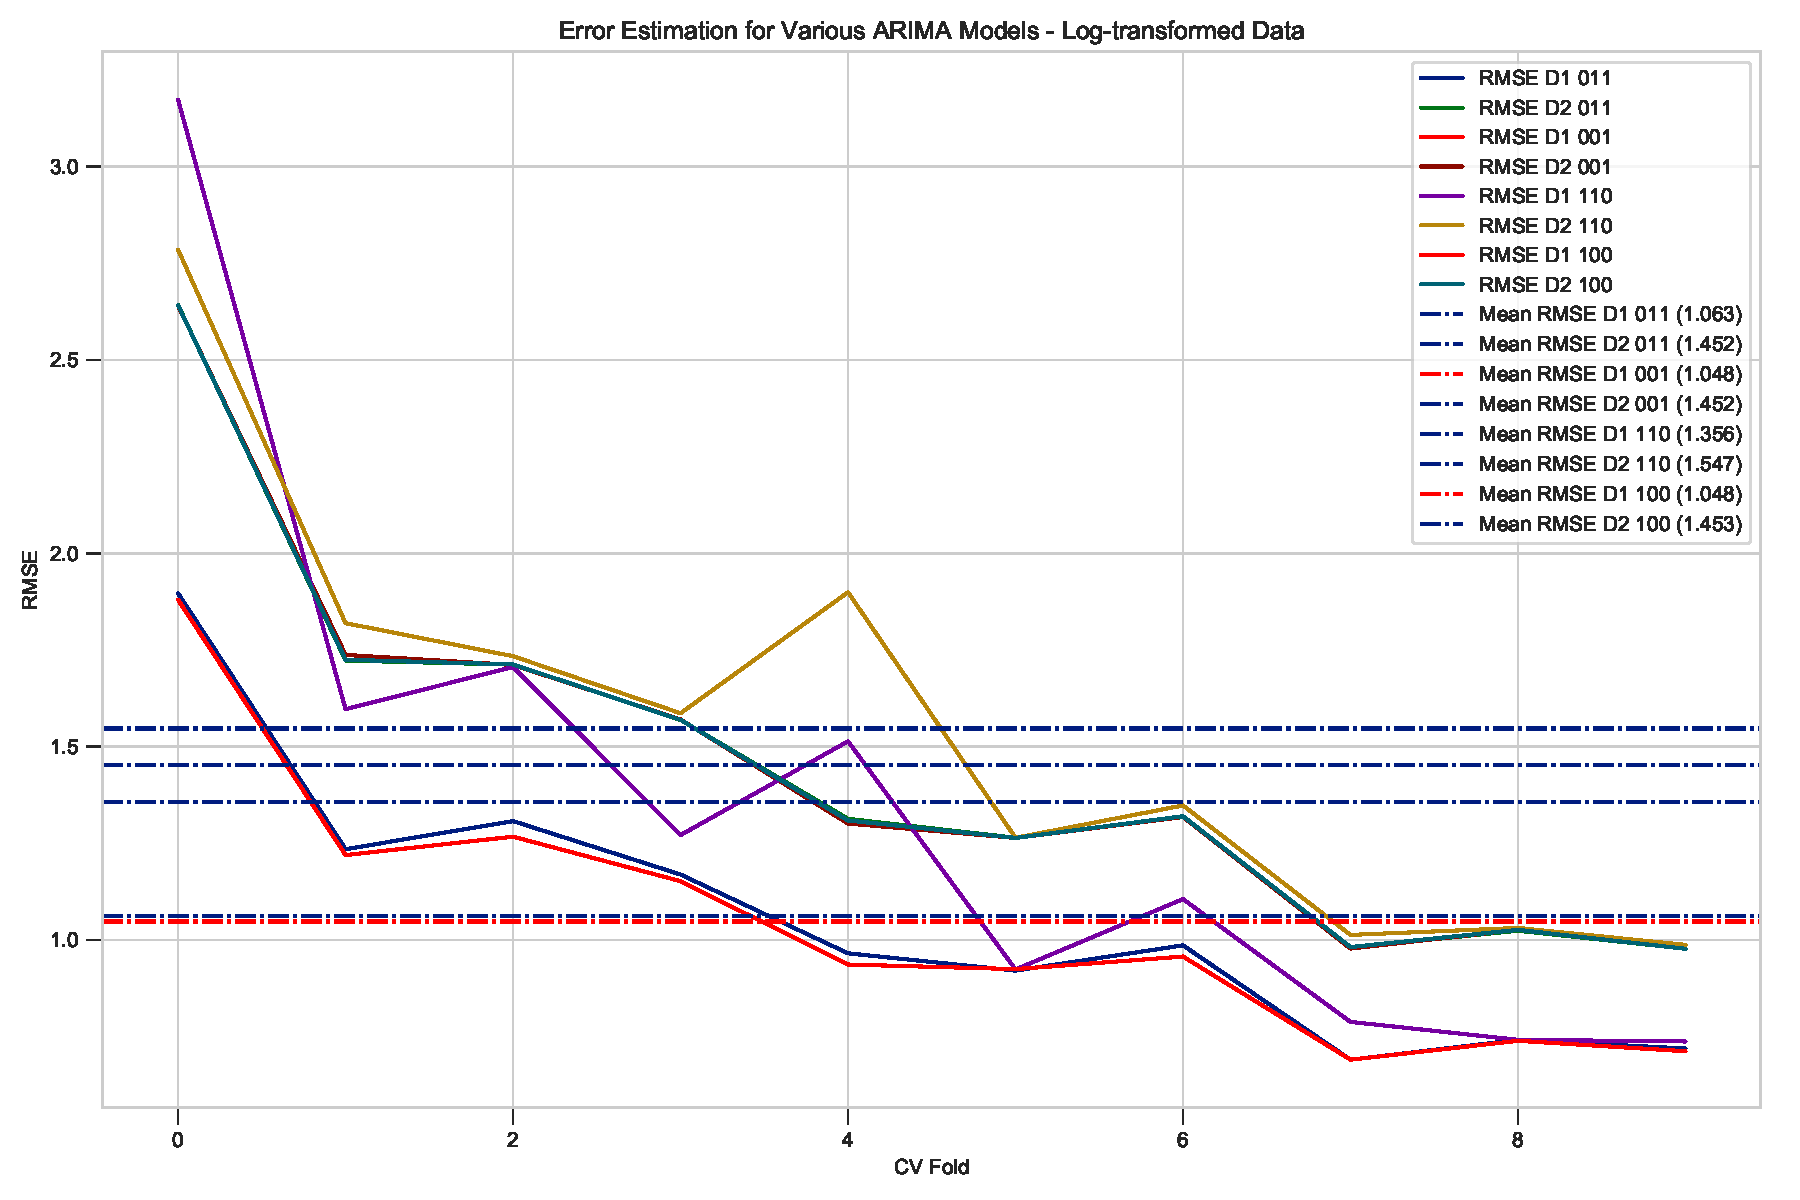
\includegraphics[width=1\columnwidth]{../Figures/error_estimation_2.pdf}
	\caption{Error Estimation on Log-transformed Data.}
	\label{fig:error_estimation_2}
\end{figure}
%

Hence ARIMA(0,1,1) is chosen to model the time series. Since the original data is not stationary, a first order differencing transformation is applied to make it stationary. The resultant time series as shown in Fig \ref{fig:data_1_d} is stationary. 
%
\begin{figure}[hbtp]
	\centering
	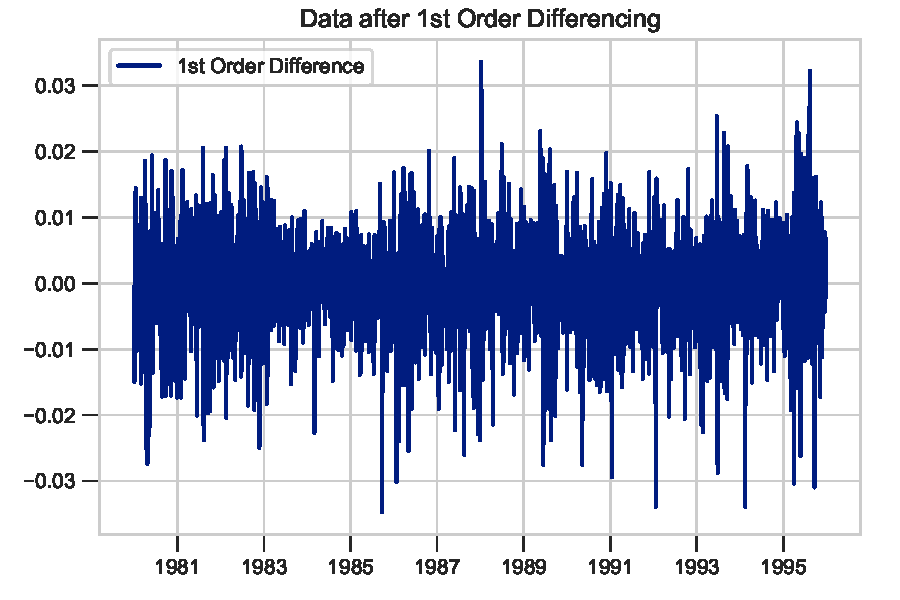
\includegraphics[width=1\columnwidth]{../Figures/data_1_d.pdf}
	\caption{Data after 1st Order Differencing.}
	\label{fig:data_1_d}
\end{figure}
%


%
\begin{figure}[hbtp]
	\centering
	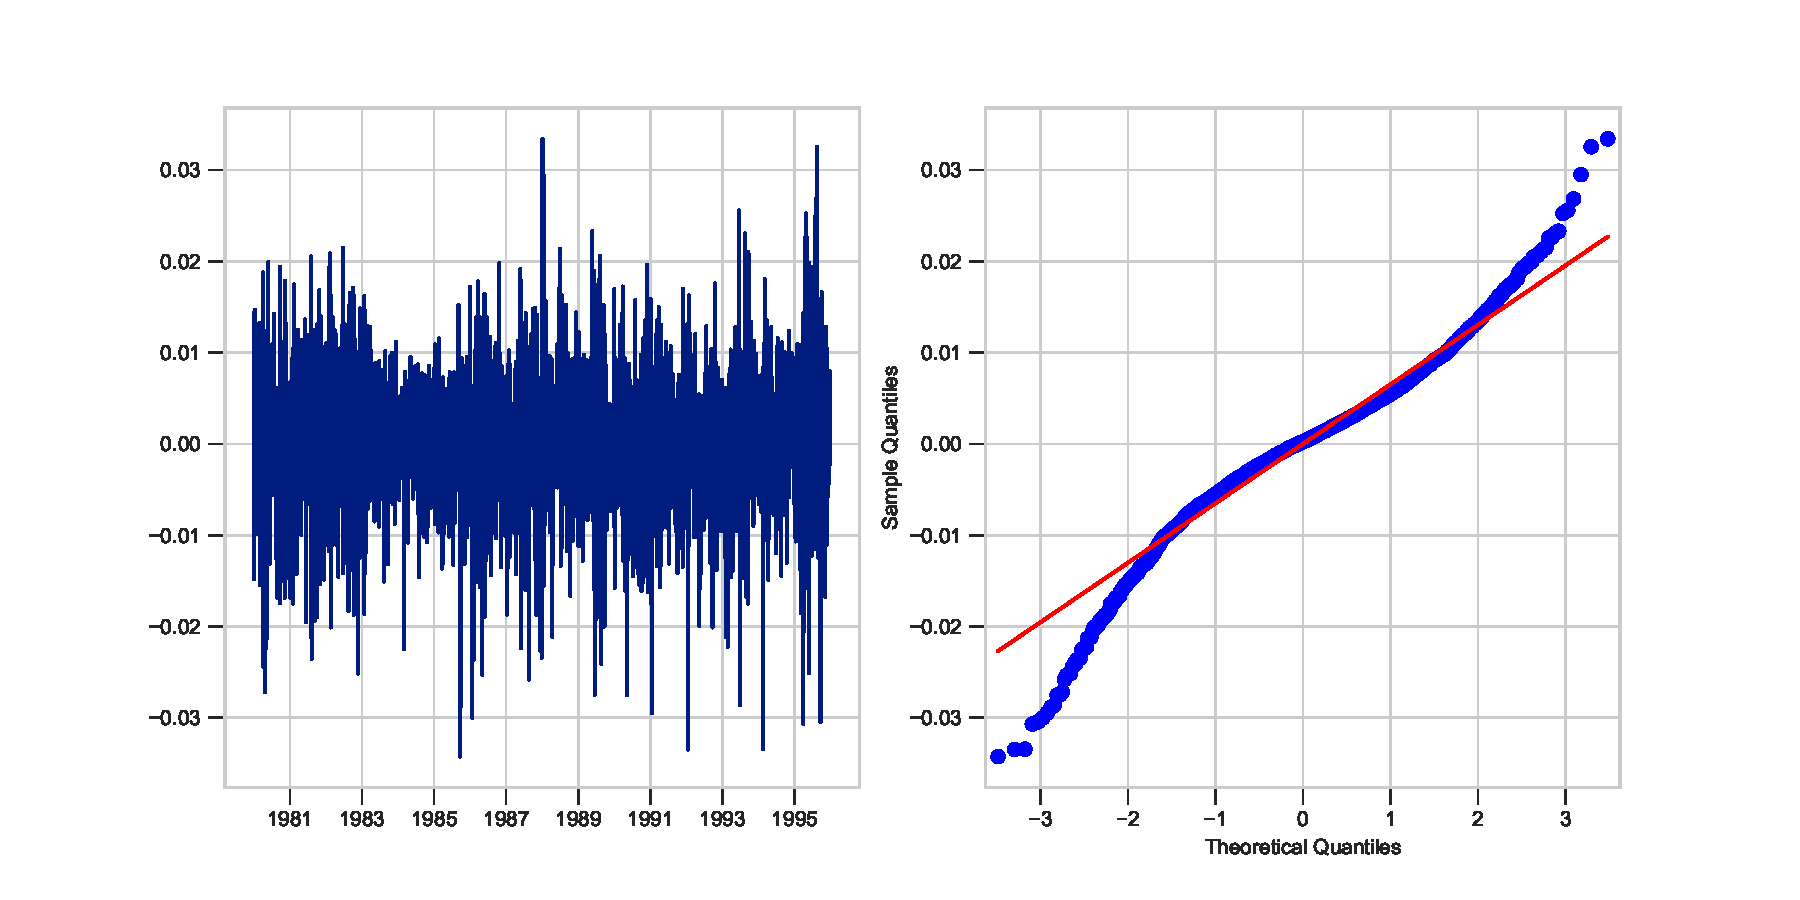
\includegraphics[width=1\columnwidth]{../Figures/res_after_arma.pdf}
	\caption{Residuals of ARIMA(0,0,1) Model.}
	\label{fig:res_after_arma}
\end{figure}
%
%
\begin{figure}[hbtp]
	\centering
	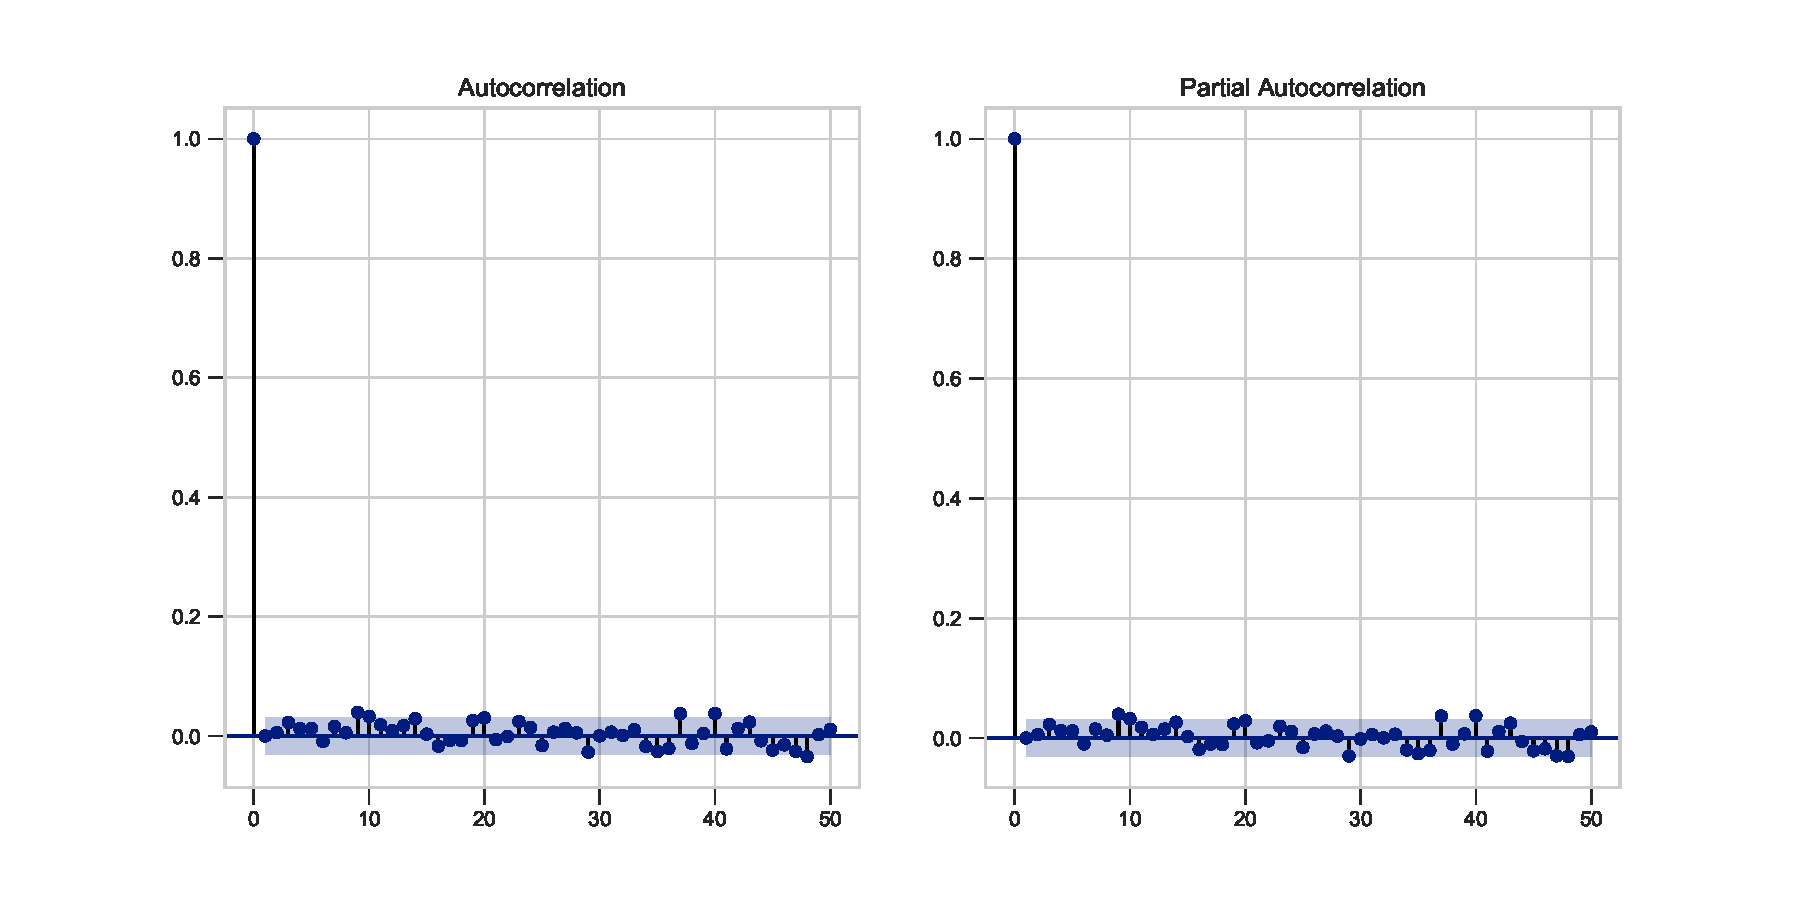
\includegraphics[width=1\columnwidth]{../Figures/sacf_n_spacf_after_arma.pdf}
	\caption{SACF and SPACF of Residuals from ARIMA(0,0,1) Model.}
	\label{fig:sacf_n_spacf_after_arma}
\end{figure}
%

\subsection{Regression on Time}
A least square regression model is developed to model the time series, initially with only time-related information. These information are year, month, day and day of the week. Also, an indicator variable to indicate whether the year is before or after 1986 where the drastic drop happens. However, this regression model does not perform well by the 10-fold cross validation rmse with a high value of 369. 

Regression on time model is not adequate enough to predict the time series, based on the 10-fold rmse, which is much higher than that of the MA(1) model on first order differenced data. Also, the error is heavily pulled up by the period where the exchange rate declined drastically during 1986. Excluding the error of that test, the average RMSE of the rest is around 24, which is still one-fold higher than the previous model.

However, with lagged data added to the predictors, the performance of the model improves tremendously. 

Result: Using single currency information, regression on lag\_1, lag2-lag1 and indicator variable performs the best, although considering uncertainties, they could be considered the same, for 10-fold cross validation in terms of rmse of 1-step-ahead forecasting. 

%
\begin{figure}[hbtp]
	\centering
	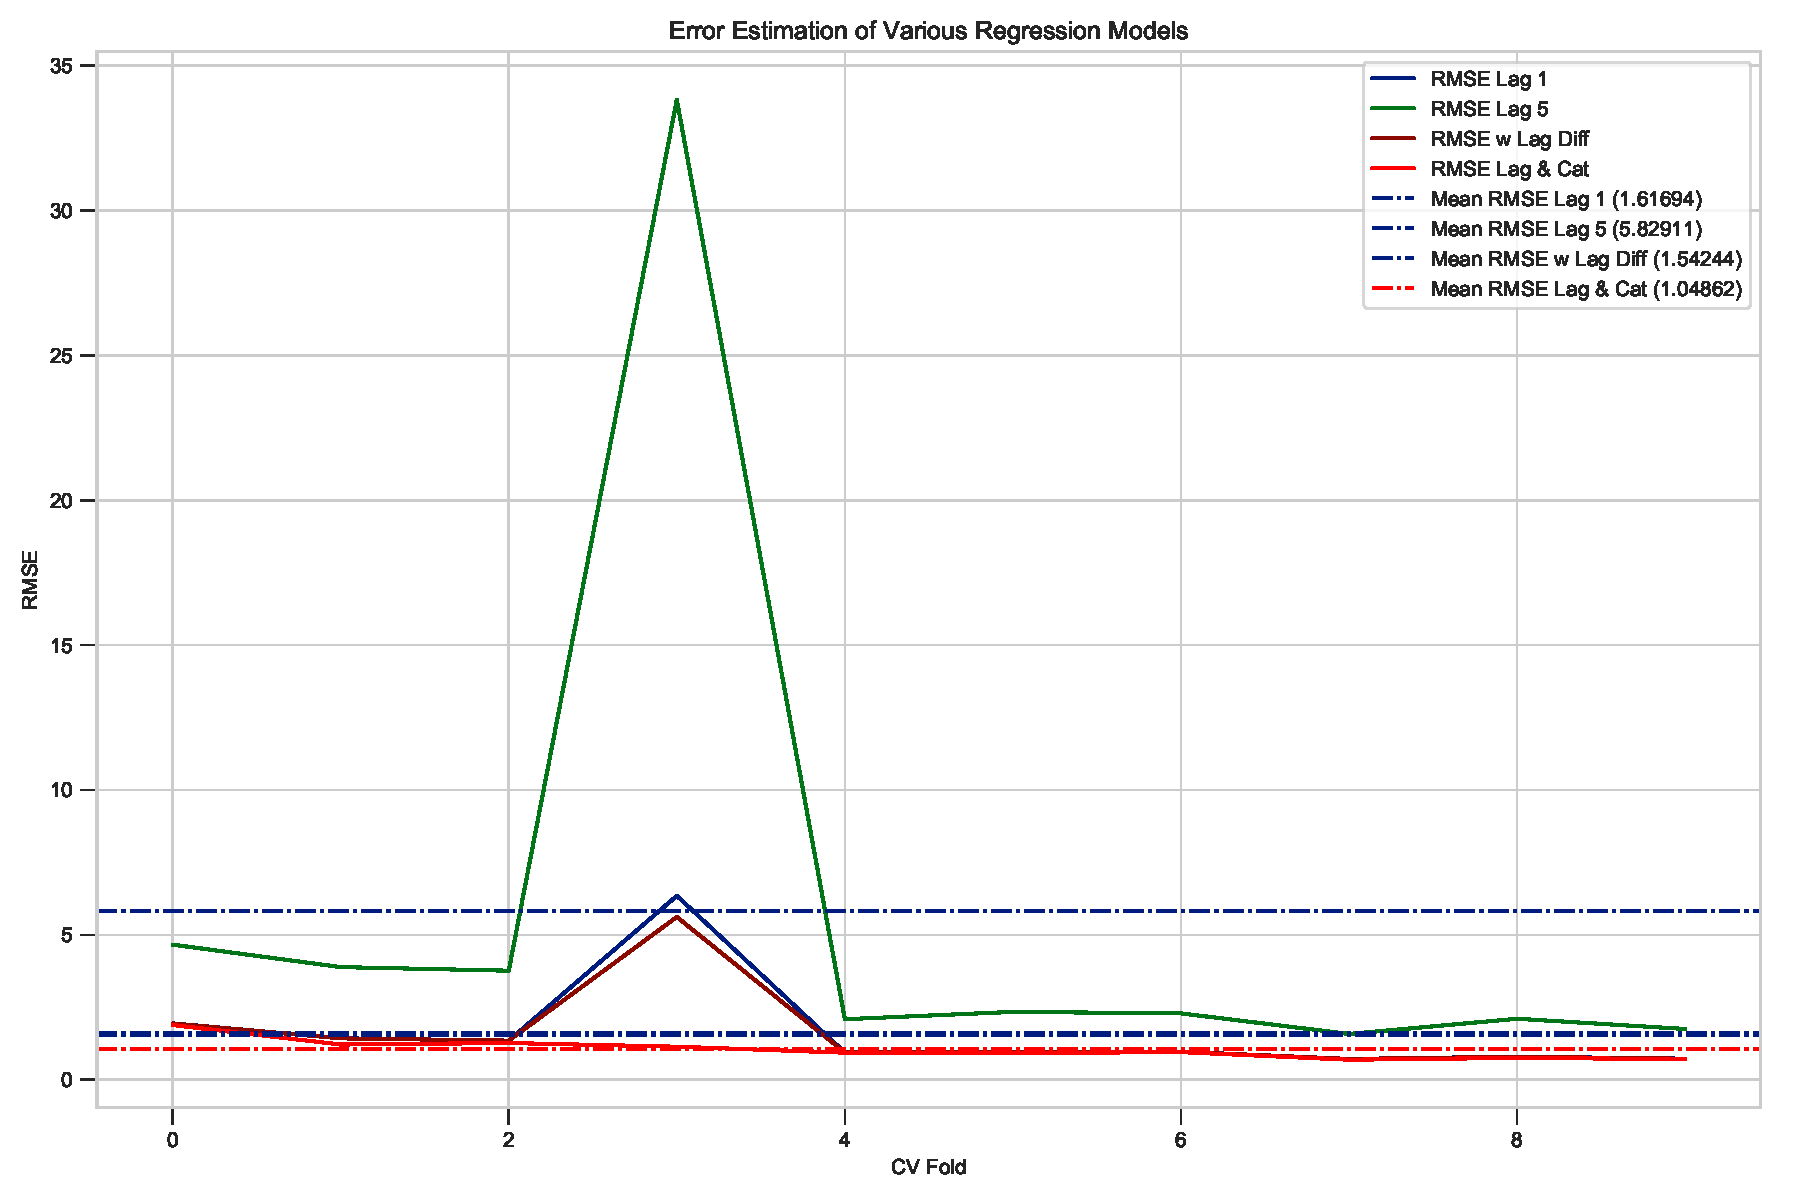
\includegraphics[width=1\columnwidth]{../Figures/error_estimation_3.pdf}
	\caption{Error Estimation of Various Regression Models.}
	\label{fig:error_estimation_3}
\end{figure}
%

The best performing model obtains the lowest RMSE of 1.048, it contains three predictors: 
\begin{itemize}
	\item Indicator variable: true if it is before 1986
	\item Difference between lag 1 value and lag 2 value
	\item Lag 1 value
\end{itemize}

\begin{center}
	\begin{tabular}{lclc}
		\toprule
		\textbf{Dep. Variable:}       &     JPY\_USD      & \textbf{  R-squared:         } &     1.000   \\
		\textbf{Model:}               &       OLS        & \textbf{  Adj. R-squared:    } &     1.000   \\
		\textbf{Method:}              &  Least Squares   & \textbf{  F-statistic:       } & 3.032e+06   \\
		\textbf{Date:}                & Sun, 19 Nov 2017 & \textbf{  Prob (F-statistic):} &     0.00    \\
		\textbf{Time:}                &     20:57:14     & \textbf{  Log-Likelihood:    } &   -6274.6   \\
		\textbf{No. Observations:}    &        4017      & \textbf{  AIC:               } & 1.256e+04   \\
		\textbf{Df Residuals:}        &        4013      & \textbf{  BIC:               } & 1.258e+04   \\
		\textbf{Df Model:}            &           3      & \textbf{                     } &             \\
		\bottomrule
	\end{tabular}
	\begin{tabular}{lcccccc}
		& \textbf{coef} & \textbf{std err} & \textbf{t} & \textbf{P$>$$|$t$|$} & \textbf{[0.025} & \textbf{0.975]}  \\
		\midrule
		\textbf{Intercept}            &       0.3044  &        0.119     &     2.551  &         0.011        &        0.070    &        0.538     \\
		\textbf{C(bef\_1986)[T.True]} &       0.2920  &        0.103     &     2.840  &         0.005        &        0.090    &        0.494     \\
		\textbf{diff\_lag\_1\_lag\_2} &       0.0316  &        0.016     &     2.004  &         0.045        &        0.001    &        0.062     \\
		\textbf{jpy\_usd\_lag\_1}     &       0.9974  &        0.001     &  1101.504  &         0.000        &        0.996    &        0.999     \\
		\bottomrule
	\end{tabular}
	\begin{tabular}{lclc}
		\textbf{Omnibus:}       & 570.043 & \textbf{  Durbin-Watson:     } &    2.001  \\
		\textbf{Prob(Omnibus):} &   0.000 & \textbf{  Jarque-Bera (JB):  } & 3070.672  \\
		\textbf{Skew:}          &  -0.563 & \textbf{  Prob(JB):          } &     0.00  \\
		\textbf{Kurtosis:}      &   7.132 & \textbf{  Cond. No.          } & 1.49e+03  \\
		\bottomrule
	\end{tabular}
	%\caption{OLS Regression Results}
\end{center}




\end{document}          
